\achapter{7}{Open Balls and Neighborhoods in Metric Spaces}\label{chap:open_balls}


\vspace*{-17 pt}
\framebox{
\parbox{\dimexpr\linewidth-3\fboxsep-3\fboxrule}
{\begin{fqs}
\item What is an open ball in a metric space? Give one important property of open balls.
\item What is a neighborhood of a point in a metric space?
\item How can we use open balls or neighborhoods to determine the continuity of a function at a point?
\end{fqs}}}

\vspace*{13 pt}

\csection{Introduction}\label{sec_open_balls_intro}
Open sets are vitally important in topology. We will see later that every topological space is completely defined by its open sets, and continuous functions can be defined just in terms of open sets. In this section we introduce the idea of open balls and neighborhoods in metric spaces and discover a few of their properties. This discussion will form the basis for introducing open sets in the next section.

Recall that the continuity of a function $f$ from a metric space $(X, d_X)$ to a metric space $(Y, d_Y)$ at a point $a$ is defined in terms of sets of points $x \in X$ such that $d_X(x,a) < \delta$ and $y \in Y$ such that $d_Y(y, f(a)) < \epsilon$ for positive real numbers $\delta$ and $\epsilon$. In $\R$ with the Euclidean metric $d_E$, for real numbers $x$ and $a$ the set of $x$ values satisfying $d_E(x,a) < \delta$ is the set of $x$ values so that $| x-a | < \delta$. We often write this set in interval notation as $(a-\delta, a+\delta)$ and call $(a-\delta, a+\delta)$ an open interval. An informal reason that we call such an interval open (as opposed to the intervals $[a-\delta, a+\delta)$, $(a-\delta, a+\delta]$, or $[a-\delta, a+\delta]$) is that the open interval does not contain either of its endpoints. A more substantial reason to call such an interval open is that if $x'$ is any element in $(a-\delta, a+\delta)$, then we can find another open interval around $x'$ that is completely contained in the interval $(a-\delta, a+\delta)$. So you could naively think of an open interval as one in which there is enough room in the interval for any point in the interval to wiggle around a bit and stay within the interval. 

Since the open interval $(a-\delta, a+\delta)$ can be described completely by the Euclidean metric as the set of $x$ values so that $d_E(x,a) < \delta$, there is no reason why we can't extend this notation of open interval to any metric space. We must note, though, that $\R$ is one-dimensional while most metric spaces are not, so the term ``interval" will no longer be appropriate. We replace the concept of interval with that of an open ball.

\begin{definition} Let $(X, d_X)$ be a metric space, and let $a \in X$. For $\delta > 0$, the \textbf{open ball} $B(a, \delta)$ \textbf{of radius $\delta$ around $a$}\index{open ball in a metric space} is the set 
\[B(a, \delta) = \{x \in X \mid d_X(x,a) < \delta\}.\]
\end{definition}

We note here that our notation for an open ball is not universal. For example, some texts use $B_{\delta}(a)$ for our $B(a,\delta)$. 

\begin{pa} Describe and draw a picture of the indicated open ball in each of the following metric spaces. 
\be
\item The open ball $B(2, 1)$ in the metric space $(\R, d_E)$ with the Euclidean metric
\[d_E(x,y) = | x-y |.\]

\item The open ball $B((3,2), 1)$ in the metric space $(\R^2, d_E)$ with the Euclidean metric
\[d_E((x_1,x_2),(y_1,y_2)) = \sqrt{(x_1-y_1)^2 + (x_2-y_2)^2}.\]


\item The open ball $B((3,2), 1)$ in the metric space $(\R^2, d_M)$ with the max metric
\[d_M((x_1,x_2),(y_1,y_2)) = \max\{| x_1-y_1 |, | x_2-y_2 |\}.\]

\item The open ball $B((3,2), 1)$ in the metric space $(\R^2, d_T)$ with the taxicab metric
\[d_T((x_1,x_2),(y_1,y_2)) = | x_1-y_1 | + | x_2-y_2 |.\]

\item The open ball $B((3,2), 1)$ in the metric space $(\R^2, d)$ with the discrete metric
\[d(x,y) = \begin{cases} 0 &\text{if } x=y \\ 1 &\text{if } x \neq y.\end{cases}.\]
What is the difference between $B((3,2),1)$ and $B((3,2),r)$ in this metric space if $r > 1$? If $r < 1$?

\ee


\end{pa}

\begin{comment}

\ActivitySolution
\be
\item  In this case the ball $B(2,1)$ is the set $\{x \mid | x-2 | < 1\}$. The solutions to the inequality $| x-2 | < 1$ are the values of $x$ so that $1 < x < 3$ as shown in Figure \ref{F:Ball_E1}. 
\begin{figure}[ht]
\begin{center}
\resizebox{!}{0.25in}{\includegraphics{Ball_E1}}
\caption{$B(2, 1)$ in $(\R, d_E)$ .}
\label{F:Ball_E1}
\end{center}
\end{figure}

\item  The open ball $B((3,2), 1)$ in this metric space is the set of points $(x,y)$ so that
\[\sqrt{(x-3)^2+(y-2)^2} < 1,\]
or 
\[(x-3)^2+(y-2)^2 < 1.\]
Since the equation $(x-3)^2+(y-2)^2 = 1$ is the equation of a circle centered at the point $(3,2)$ with radius 1, the open ball $B((3,2), 1)$ is the set of all points inside the disk whose boundary is this circle as illustrated at left in Figure \ref{F:Balls_2_3}.

\begin{figure}[ht]
\begin{center}
\resizebox{!}{2.0in}{\includegraphics{Ball_E2}} \hspace{0.25in}
\resizebox{!}{2.0in}{\includegraphics{Ball_M}} 
\caption{Left: $B((3,2), 1)$ in $(\R^2, d_E)$. Right: $B((3,2), 1)$ in $(\R, d_M)$.}
\label{F:Balls_2_3}
\end{center}
\end{figure}



%\begin{figure}[ht]
%\begin{center}
%\begin{minipage}{3in} 
%\begin{center}
%\resizebox{!}{2.0in}{\includegraphics{Ball_E2}} 
%\caption{$B((3,2), 1)$ in $(\R^2, d_E)$.}
%\label{F:Ball_E2}
%\end{center}
%\end{minipage} \hspace{0.25in}
%\begin{minipage}{3in}
%\begin{center}
%\resizebox{!}{2.0in}{\includegraphics{Ball_M}} 
%\caption{$B((3,2), 1)$ in $(\R, d_M)$.}
%\label{F:Ball_M}
%\end{center}
%\end{minipage}
%\end{center}
%\end{figure}


\item  The open ball $B((3,2), 1)$ in this metric space is the set of points $(x,y)$ so that
\[\max\{| x-3 |, | y-2 |\} < 1.\]
This will happen when 
\[| x-3 | < 1 \ \text{ or } \ | y-2 | < 1,\]
giving us the set of points $(x,y)$ such that $2<x<4$ and $1<y<3$. This describes the inside of the box whose sides are bounded by the lines $x=2$, $x=4$, $y=1$, and $y=3$ as illustrated at right in Figure \ref{F:Balls_2_3}.
%\begin{figure}[ht]
%\begin{center}
%\resizebox{!}{2.0in}{\includegraphics{Ball_M}} 
%\caption{$B((3,2), 1)$ in $(\R, d_M)$.}
%\label{F:Ball_M}
%\end{center}
%\end{figure}

\item  The open ball $B((3,2), 1)$ in this metric space is the set of points $(x,y)$ so that
\[| x-3 | + | y-2 | < 1.\]
The equation $| x-3 | + | y-2 | = 1$ has as its solution the four lines 
\begin{align*}
(x-3) + (y-2) &= 1 \\
(x-3) + (2-y) &= 1 \\
(3-x) + (y-2) &= 1 \\
(3-x) + (2-y) &= 1.
\end{align*}
The graphs of these four lines 
\begin{align*}
x+y &= 6 \\
x-y &= 2 \\
y-x &= 0  \\
x+y &= 4.
\end{align*}
These four lines form the diamond shown in Figure \ref{F:Balls_4_5}, and so the open ball $B((3,2), 1)$ in this metric space is the inside of that diamond as illustrated at left in Figure \ref{F:Balls_4_5}.

\begin{figure}[ht]
\begin{center}
\resizebox{!}{2.0in}{\includegraphics{Ball_T}} \hspace{0.25in} 
\resizebox{!}{2.0in}{\includegraphics{Ball_D}} 
\caption{Left: $B((3,2), 0.5)$ in $(\R^2, d_T)$. Right: $B((3,2), 1)$ in $(\R^2, d)$.}
\label{F:Balls_4_5}
\end{center}
\end{figure}


%\begin{figure}[ht]
%\begin{center}
%\resizebox{!}{2.0in}{\includegraphics{Ball_T}} 
%\caption{$B((3,2), 0.5)$ in $(\R^2, d_T)$.}
%\label{F:Ball_T}
%\end{center}
%\end{figure}

%\begin{figure}[ht]
%\begin{center}
%\begin{minipage}{3in} 
%\begin{center}
%\resizebox{!}{2.0in}{\includegraphics{Ball_T}} 
%\caption{$B((3,2), 0.5)$ in $(\R^2, d_T)$.}
%\label{F:Ball_T}
%\end{center}
%\end{minipage} \hspace{0.25in}
%\begin{minipage}{3in}
%\begin{center}
%\resizebox{!}{2.0in}{\includegraphics{Ball_D}} 
%\caption{$B((3,2), 1)$ in $(\R^2, d)$.}
%\label{F:Ball_D}
%\end{center}
%\end{minipage}
%\end{center}
%\end{figure}

\item  Let $a = (3,2)$. If $x \neq a$ in this space, then $d(x,a) = 1$. So the only element in $B((3,2),1)$ in this space is $a$ itself, as shown at right in Figure \ref{F:Balls_4_5}. However, if $r > 1$, then every element in $\R^2$ is in $B(a,r)$. 
%\begin{figure}[ht]
%\begin{center}
%\resizebox{!}{2.0in}{\includegraphics{Ball_D}} 
%\caption{$B((3,2), 1)$ in $(\R^2, d)$.}
%\label{F:Ball_D}
%\end{center}
%\end{figure}

\ee

\end{comment}


\csection{Neighborhoods}\label{sec_neighborhoods}

We are familiar with the idea of open intervals in $\R$. We next introduce the idea of an open neighborhood of a point and characterize continuity in terms of neighborhoods. This is the next step in developing the notation of continuity in topological spaces. 

The open ball $B(a, \delta)$ in a metric space $(X,d)$ is also called the \emph{$\delta$-neighborhood}\index{$\delta$-neighborhood of a point in a metric space} around $a$. A neighborhood of a point can be thought of as any set that envelops that point. 

\begin{definition} Let $(X, d_X)$ be a metric space, and let $a \in X$. A subset $N$ of $X$ is a \textbf{neighborhood}\index{neighborhood in a metric space} of $a$ if there exists a $\delta > 0$ such that $B(a, \delta) \subseteq N$. 
\end{definition} 

\begin{example} \label{exp:neighborhood_MS} ~
\begin{itemize}
\item In $\R$ with the Euclidean metric, the set $\R^+$ (the positive real numbers) is a neighborhood of $a=1$ because the open ball $B(1,0.5)$ is completely contained in $\R^+$.  
\item In $\R$ with the Euclidean metric, the set $\Z$ is not a neighborhood of $a=1$ because any open ball centered at $a=1$ will contain some non-integers. 
\item In $\R$ with the discrete metric, the set $\Z$ is a neighborhood of $a=1$ because the open ball $B(a,1) = \{a\}$. 
\end{itemize}

\end{example}
 
As another example, the open ball $B(a, \delta)$ is a neighborhood of $a$. We can say even more about open balls. 

\begin{activity} Let $(X, d)$ be a metric space, let $a \in X$, and let $\delta > 0$.  In this activity we ask the question, is $B(a, \delta)$ a neighborhood of each of its points? 
\ba
\item Let $b \in B(a, \delta)$. What do we have to do to show that $B(a, \delta)$ is a neighborhood of $b$? 

\item Use Figure \ref{F:Open_ball_neighborhood} to help show that $B(a, \delta)$ is a neighborhood of $b$.
\begin{figure}[h]
\begin{center}
\resizebox{!}{2.0in}{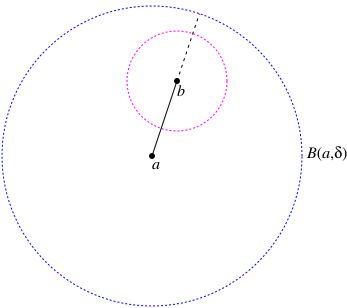
\includegraphics{Open_ball_neighborhood}}
\caption{$B(a, \delta)$ as a neighborhood of $b$.} 
\label{F:Open_ball_neighborhood}
\end{center}
\end{figure}

\item Is the converse true? That is, if a set is a neighborhood of each of its points, is the set an open ball? No proof is necessary, but a convincing argument is in order. 

\ea

\end{activity}

\begin{comment}

\ActivitySolution
\ba
\item We need to show that there is an open ball around $b$ that is entirely contained in $B(a, \delta)$. 


\item Let $\beta = d(a,b)$ and let $\gamma = \delta - \beta$. Let $c \in B(b,\gamma)$. Then 
\[d(a,c) \leq d(a,b) + d(b,c) < \beta + \gamma = \beta + (\delta - \beta) = \delta.\]
So $c \in B(a,\delta)$ and $B(b,\gamma) \subset B(a,\delta)$.  

\item This statement is not true. Consider $A = (0,1) \cup (2,3)$ as a subset of $\R$ with the Euclidean metric. The set $A$ is a neighborhood of each of its points, but $A$ is not an open ball -- rather $A$ is the union of two disjoint open balls. 

\ea

\end{comment}

\csection{Continuity and Neighborhoods}\label{sec_cont_neighborhoods}
We can define continuity now in terms of neighborhoods instead of using metrics. The advantage here is that this idea does not explicitly depend on the existence of a metric, so we will be able to adopt this concept of continuity for arbitrary topological spaces. 

Recall that a function $f$ from a metric space $(X, d_X)$ to a metric space $(Y, d_Y)$ is continuous at $a \in X$ if, for any $\epsilon > 0$ there exists $\delta > 0$ so that $d_X(x,a) < \delta$ implies $d_Y(f(x),f(a)) < \epsilon$. We can interpret this definition of continuity to say that for every $\epsilon > 0$, the inverse image under $f$ of the open ball $B(f(a), \epsilon)$ contains the open ball $B(a, \delta)$ for some $\delta > 0$. It is not unreasonable to wonder if the set $f^{-1}\left(B(f(a), \epsilon)\right)$ itself is an open ball. We investigate this question in the following activity. 

\begin{activity} \label{act:OB_1} Let $f$ be a function from a metric space $(X, d_X)$ to a metric space $(Y, d_Y)$ that is continuous at $a \in X$. Using the notation from the paragraph above, in this activity we determine if $f^{-1}\left(B(f(a), \epsilon)\right)$ must equal $B(a, \delta)$ for some $\delta$.

Define $f : \R \to \R$ by 
\[f(x) = x^2,\]
where we use the Euclidean metric $d_E$ throughout.  Assume that $f$ is a continuous function.  Then $f$ is continuous at $x=2$.
\ba
\item What is $B(f(2), 1)$? 

\item What is $f^{-1}\left(B(f(2), 1)\right)$?

\item Is $f^{-1}\left(B(f(2), 1)\right)$ an open ball centered at $2$? Explain.

\ea

\end{activity}
 
\begin{comment}

\ActivitySolution
\ba
\item The set $B(f(2),1)$ is the interval $(f(2)-1,f(2)+1) = (3,5)$ in $\R$.

\item The set of points in $\R$ that map into $B(f(2),1)$ is the interval $(\sqrt{3}, \sqrt{5})$. 

\item Since $\sqrt{5} - 2 \approx 0.236$ and $2 - \sqrt{3} \approx 0.2679$, the set $f^{-1}\left(B(f(2), 1)\right)$ only contains an open ball centered at $2$, but is not itself an open ball centered at 2. 

\ea

\end{comment}

The conclusion to be drawn from Activity \ref{act:OB_1} is that if $f$ is continuous, we can only conclude that the inverse image of $B(f(a), \epsilon)$ \emph{contains} an open ball centered at $a$. By definition of continuity, if for every $\epsilon > 0$ there exists a $\delta > 0$ so that the open ball $f^{-1}\left(B(f(a), \epsilon)\right)$ contains $B(a, \delta)$, then $f$ is continuous at $a$. We summarize this in the next theorem.


\begin{theorem} \label{thm:open_ball_continuity} Let $f$ be a function a metric space $(X, d_X)$ to a metric space $(Y, d_Y)$, and let $a \in X$. Then $f$ is continuous at $a \in X$ if and only if, given any $\epsilon > 0$ there exists $\delta > 0$ so that 
\[B(a, \delta) \subseteq f^{-1}\left(B(f(a), \epsilon)\right).\]
\end{theorem}

We can extend this idea of continuity to describe continuity in terms of neighborhoods. This condition will allow us to later consider continuous functions even if there are no metrics on our spaces. 

\begin{theorem} Let $(X, d_X)$ and $(Y,d_Y)$ be metric spaces, and let $f : X \to Y$ be a function. Then $f$ is continuous at $a \in X$ if and only if the inverse image of every neighborhood of $f(a)$ is a neighborhood of $a$. 
\end{theorem}

\begin{proof} Let $(X, d_X)$ and $(Y,d_Y)$ be metric spaces, and let $f : X \to Y$ be a function. To prove this biconditional statement we need to prove both implications. First assume that $f$ is continuous at some point $a \in X$. We will show that for any neighborhood $N$ of $f(a)$ in $Y$, its inverse image $f^{-1}(N)$ in $X$ is a neighborhood of $a$ in $X$. Let $N$ be a neighborhood of $f(a)$ in $Y$. To demonstrate that $f^{-1}(N)$ is a neighborhood of $a$ in $X$, we need to find an open ball around $a$ that is contained in $f^{-1}(N)$. Since $N$ is a neighborhood of $f(a)$, by definition there exists $\epsilon > 0$ so that $B(f(a), \epsilon) \subseteq N$. Since $f$ is continuous at $a$, there exists $\delta > 0$ such that $B(a, \delta) \subseteq f^{-1}\left(B(f(a), \epsilon)\right)$. So if $x \in B(a, \delta)$, then $f(x) \in B(f(a), \epsilon) \subseteq N$. So $B(a, \delta) \subseteq f^{-1}(N)$, and $f^{-1}(N)$ is a neighborhood of $a$ in $X$. 

The proof of the reverse implication is left for the next activity.
\end{proof}



\begin{activity} Let $(X, d_X)$ and $(Y,d_Y)$ be metric spaces, and let $f : X \to Y$ be a function. Let $a \in X$. In this activity we prove that if the inverse image of every neighborhood of $f(a)$ is a neighborhood of $a$, then $f$ is continuous at $a$.
\ba
\item What does Theorem \ref{thm:open_ball_continuity} tell us that we need to do to show that $f$ is continuous at $a$?

\item Suppose $\epsilon$ is greater than 0, why is $B(f(a), \epsilon)$ a neighborhood of $f(a)$ in $Y$?

\item What does our hypothesis tell us about $f^{-1}\left(B(f(a), \epsilon)\right)$?

\item What can we conclude from part (c)?

\item How do (a)-(d) show that $f$ is continuous at $a$?

\ea

\end{activity}

\begin{comment}

\ActivitySolution
\ba
\item We need to show that the inverse image of any open ball centered at $f(a)$ contains an open ball centered at $a$.

\item We showed earlier that an open ball is a neighborhood of each of its points.

\item Our hypothesis tells us that $f^{-1}\left(B(f(a), \epsilon)\right)$ is a neighborhood of $a$ in $X$. 

\item As a neighborhood of $a$, it follows that there exists $\delta > 0$ such that $B(a, \delta) \subseteq f^{-1}\left(B(f(a), \epsilon)\right)$. 

\item The previous parts show that given any $\epsilon > 0$ there exists $\delta > 0$ such that $B(a, \delta) \subseteq f^{-1}\left(B(f(a), \epsilon)\right)$. Theorem \ref{thm:open_ball_continuity} then shows that $f$ is continuous at $a$. 

\ea

\end{comment}

\noindent We conclude this section with some important facts about neighborhoods. Assume that $(X,d)$ is a metric space and $a \in X$. 

\begin{itemize}
\item There is a neighborhood that contains $a$.
\item If $N$ is a neighborhood of $a$ and $N \subseteq M$, then $M$ is a neighborhood of $a$.
\item If $M$ and $N$ are neighborhoods of $a$, then so is $M \cap N$.
\end{itemize}

The proofs are straightforward and left for Exercise (\ref{ex:Nghb_properties}).

\csection{Summary}\label{sec_open_balls_summ}
Important ideas that we discussed in this section include the following.
\begin{itemize}
\item If $(X,d)$ is a metric space and $a \in X$, then an open ball centered at $a$ is a set of the form
\[B(a,\delta) = \{ x \in X \mid d(x,a) < \delta\}\]
for some positive number $\delta$. 
\item A subset $N$ of a metric space $(X,d)$ is s neighborhood of a point $a \in N$ if there is a positive real number $\delta$ such that $B(a,\delta) \subseteq N$.
\item An important property of open balls is that every open ball is a neighborhood of each of its points. This is our first step toward defining the concept of open sets that will form the foundation for topological spaces. 
\item A function $f$ from a metric space $(X,d_X)$ to a metric space $(Y,d_Y)$ is continuous at $a \in X$ if $f^{-1}(N)$ is a neighborhood of $a$ in $X$ for any neighborhood $N$ of $f(a)$ in $Y$. 
\end{itemize}


\csection{Exercises}\label{sec_open_balls_exer}

\be

\item Determine, with proof, which of the following sets $A$ is a neighborhood of $a$ in the indicated metric space. 

\ba

\item $A = \{(x,y) \in \R^2 \mid x^2+y^2 < 1\}$ in $(\R^2,d_E)$ with $a = (0.5,0.5)$

\item $A$ is the $x$-axis in $(\R^2,d_T)$ with $a =(0,0)$, where $d_T$ is the taxicab metric

\item $A$ is the set of rational numbers in $(\R, d_E)$ with $a = 0$

\item $A$ is the set of positive integers in $(Q,d)$ and $a = 1$, where $Q$ is the set of all rational numbers in reduced form with metric $d : Q \times Q \to \R$ defined by 
\[d\left(\frac{a}{b}, \frac{c}{d}\right) = \max\{| a-c |, | b-d |\}\]
(The fact that $d$ is a metric is the topic of Exercise \ref{ex:MS_Q_metric} on page \pageref{ex:MS_Q_metric}.)


\ea

\begin{comment}

\ExerciseSolution

\ba

\item Since $A = B((0,0),1)$ and we know that every open ball is a neighborhood of each of its points, we conclude that $A$ is a neighborhood of $a$. 

\item Let $\delta$ be a positive real number and consider the open ball $B(a, \delta)$ in $(\R^2,d_T)$. The point $\left(0, \frac{\delta}{2}\right)$ is in $B(a,\delta)$ but not in $A$. So $A$ cannot contain any open ball centered at $a$. We conclude that $A$ is not a neighborhood of $a$.  

\item Exercise \ref{ex:GLB_irrational} on page \pageref{ex:GLB_irrational} tells us that there is an irrational number between any two real numbers. So there are irrational numbers in any interval of the form $(a - \delta, a+\delta)$ for any $\delta > 0$. We conclude that $A$ is not a neighborhood of $a$. 

\item Consider the ball $B(a,1)$ in $Q$. An element $\frac{p}{q}$ is in $B(a,1)$ if 
\[d\left(\frac{1}{1}, \frac{p}{q}\right) = \max\{| 1-p |, | 1-q |\} < 1.\]
This can only happen if $|1-p| < 1$ and $|1-q| < 1$. But $p$ and $q$ are integers, so we must have $p = q = 1$. Thus, $B(a,1) = \{a\}$. So any set that contains $a$ in $Q$ contains $B(a,1)$. We conclude that any set that contains $a$ is a neighborhood of $a$.   

\ea

\end{comment}


\item Let $X = \{1,3,5\}$ and define $d_X: X \times X \to \R$ by $d_X(x,y) = xy - 1 \pmod{8}$. That is, $d_X(x,y)$ is the remainder when $xy - 1$ is divided by $8$. That $d_X$ is a metric on $X$ is examined in Exercise \ref{ex:MS_mod_metric} on page \pageref{ex:MS_mod_metric}. Let $(Y,d_Y)$ be a metric space. Is it possible to define a function $f: X \to Y$ that is not continuous? Explain. 

\begin{comment}

\ExerciseSolution Recall that $d_X$ has values as in Table \ref{T:open_balls_example_8}.
\begin{table}[h]
\begin{center}
\begin{tabular}{|c|c|c|c|} \hline
	&$1$	&$3$	&$5$	\\ \hline
$1$	&$0$	&$2$	&$4$	\\ \hline
$3$	&$2$	&$0$	&$6$	\\ \hline
$5$	&$4$	&$6$	&$0$	\\ \hline
\end{tabular}
\caption{Values of $d_X$.}
\label{T:open_balls_example_8}
\end{center}	
\end{table}
Notice that $B(x,1) = \{x\}$ for every $x \in X$. So if $f: X \to Y$ is a function and $N$ is a neighborhood of $f(x)$ in $Y$, then $B(x,1) \subseteq f^{-1}(N)$. So $f^{-1}(N)$ is a neighborhood of $x$ for every $x \in X$ and $f$ must be a continuous function. 

\end{comment}
	

\item If $x = (x_1, x_2, \ldots, x_n)$, we let $|x| = \sqrt{x_1^2+x_2^2+ \cdots + x_n^2}$. For $x = (x_1, x_2, \ldots, x_n)$ and $y = (y_1, y_2, \ldots y_n)$, define $d_H: \R^n \times \R^n \to \R$ by 
\[d_H(x,y) = \begin{cases} 0 &\text{ if } x=y \\ |x|+|y| &\text{ otherwise}. \end{cases}\]
The fact that $d_H$ is a metric is examined in Exercise \ref{ex:MS_hub} on page \pageref{ex:MS_hub}. 

Let $(X,d_X) = (\R^2, d_H)$ and let $(Y,d_Y) = (\R, d_E)$. Define $f: X \to Y$ and $g: X \to Y$ by 
\[f(x) = \begin{cases} 0 &\text{ if } x = (0,0) \\ 1 &\text{ otherwise} \end{cases} \  \text{ and } \ g(x) = \begin{cases} 0 &\text{ if } |x|<1 \\ 1 &\text{ otherwise} \end{cases}.\]
One of $f$, $g$ is continuous and the other is not. Determine which is which, with proof for each. 

\begin{comment}

\ExerciseSolution Let $B = B(0,1)$ in $Y$. Notice that $f^{-1}(B) = \{(0,0)\}$. Now $B((0,0),r) = \{x \in \R^2 \mid |x|<r\}.$ So the only way $B((0,0),r) = f^{-1}(B)$ is if $r=0$. Thus, $f^{-1}(B)$ is not a neighborhood of $(0,0)$ and so $f$ is not continuous. 

Now we show that $g$ is continuous. Let $a = (a_1,a_2) \in X$. We demonstrate that $g$ is continuous at $a$. By the definition of $g$, we either have $g(a) = 0$ or $g(a) = 1$. We consider the cases.
\begin{description}
\item[Case 1: $g(a) = 0$.] In this case we have $|a| < 1$. Let $B = B(g(a),\epsilon) = B(0,\epsilon) = (-\epsilon, \epsilon)$. Let $\delta = \frac{3|a|}{2}$. If $x$ is in $B(a,\delta)$, then 
\begin{align*}
d_H(a,x) &< \delta \\
|a|+|x| &<  \frac{3|a|}{2} \\
|x| &< \frac{|a|}{2} < 1.
\end{align*}
So we must have $g(x) = 0$ as well. Thus,
\[|g(a) - g(x)| = |0-0|  = 0 <  \epsilon.\]
We conclude that $g$ is continuous at $a$ when $g(a) = 0$. 
    
\item[Case 2: $g(a) = 1$.] Here we have $|a| \geq 1$. Let $\delta = |a|$. If $x$ is in $B(a,\delta)$, then 
\begin{align*}
d_H(a,x) &< \delta \\
|a|+|x| &<  |a| \\
|x| < 0.
\end{align*}
But then $B(a,\delta) = \{a\}$ and $B(a,\delta) \subseteq g^{-1}(B(g(a),\epsilon)$. We conclude that $g$ is continuous at $a$ when $g(a) = 1$. 
\end{description} 

\end{comment}

\item Recall from Section \ref{sec:metric_spaces} that we can construct a finite metric space by starting with a finite set of points and making a graph with the points as vertices. We construct edges so that the graph is connected (that is, there is a path from any one vertex to any other) and give weights to the edges. We then define a metric $d$ on $S$ by letting $d(x,y)$ be the length of a shortest path between vertices $x$ and $y$ in the graph. \\

Consider the metric space $(X,d)$ corresponding to the graph in Figure \ref{F:Graph_metric_ex}. 
\begin{figure}[h]
\begin{center}
\resizebox{!}{2.0in}{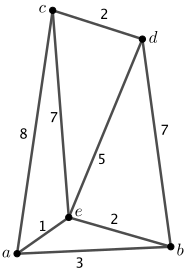
\includegraphics{Graph_metric.eps}}
\caption{A graph to define a metric.} 
\label{F:Graph_metric_ex}
\end{center}
\end{figure}
\ba
\item Determine all of the open balls $B(a,\delta)$ for every positive real number $\delta$. 

\item Find all of the neighborhoods of $a$. 

\ea

\begin{comment}

\ExerciseSolution

\ba

\item First we list the distances from $a$ to the other points in $X$:
\begin{center}
\begin{tabular}{c|cccc}
$x$		&$b$	&$c$&$d$&$e$ \\
$d(a,x)$	&$3$&$8$&$6$&$1$
\end{tabular}
\end{center}
So 
\begin{itemize}
\item if $\delta \leq 1$, then $B(a,\delta) = \{a\}$; \\
\item if $1< \delta \leq 3$, then $B(a,\delta) = \{a,e\}$; \\
\item if $3< \delta \leq 6$, then $B(a,\delta) = \{a,b,e\}$; \\
\item if $6< \delta \leq 8$, then $B(a,\delta) = \{a,b,d,e\}$; \\
\item if $8< \delta$, then $B(a,\delta) =X$.
\end{itemize}

\item Every neighborhood of $a$ must contain $a$, and if $A$ is a subset of $X$ that contains $a$, then $B(a,1) = \{a\}$ is a subset of $A$. So the neighborhoods of $a$ are the subsets of $X$ that contain $a$.  

\ea

\end{comment}

\item \label{ex:linear_continuous}
	\ba
	\item Let $f: (\R,d_E) \to (\R,d_E)$ be defined by $f(x) = ax+b$ for some real numbers $a$ and $b$ with $a \neq 0$. Let $p \in \R$ and let $r > 0$. Show that $f^{-1}(B(f(p),r))$ contains an open ball centered at $p$. Conclude that every linear function from $(\R,d_E)$ to $(\R,d_E)$ is continuous. (Hint: By Exercise \ref{ex:sum_continuous} on page \pageref{ex:sum_continuous} we can assume $a > 0$ to simplify the problem.)
	
	\item Let $f: (\R,d_E) \to (\R,d_E)$ be defined by $f(x) = ax^2+bx+c$ for some real numbers $a$, $b$, and $c$ with $a \neq 0$. Let $p \in \R$ and let $r > 0$. $f^{-1}(B(f(p),r))$ contains an open ball centered at $p$. Conclude that every quadratic function from $(\R,d_E)$ to $(\R,d_E)$ is continuous. (Hint: Consider cases.)
	
	\ea
	
\begin{comment}

\ExerciseSolution

\ba

\item Let $f(x) = ax+b$ for some real numbers $a$ and $b$ with $a > 0$. Let $p \in \R$ and let $r > 0$. Then $f^{-1}(B(f(p),r) = B\left(p, \frac{r}{m}\right)$ and so $f$ is continuous at $x=p$. Since $f$ is continuous at every real input, $f$ is a continuous function. 

\item Let $f(x) = ax^2+bx+c$ for some real numbers $a$, $b$, and $c$ with $a > 0$. Notice that $f$ attains its minimum value of $f(m) = c-\frac{b^2}{4a}$ at $m = -\frac{b}{2a}$. Let $p \in \R$ and let $r > 0$. We consider cases.
\begin{description}
\item[$p > m$:] Let $r' = \min\{r, |f(p)-f(m)|\}$. Then $B(f(p),r') \subseteq B(f(p),r)$ and $f^{-1}(B(f(p),r')) \subseteq (m, \infty)$. So there exist unique $x_1$, $x_2$ in $(m, \infty)$ such that $f(x_1) = f(p)-r'$ and $f(x_2) = f(p)+r'$. Let $s = \min\{p-x_1, x_2-p\}$. Then $B(p,s) \subseteq f^{-1}(B(f(p), r') \subseteq f^{-1}(B(f(p), r)$. 

\item[$p < m$:] Let $r' = \min\{r, |f(p)-f(m)|\}$. Then $B(f(p),r') \subseteq B(f(p),r)$ and $f^{-1}(B(f(p),r')) \subseteq (-\infty,m)$. So there exist unique $x_1$, $x_2$ in $(m, \infty)$ such that $f(x_1) = f(p)+r'$ and $f(x_2) = f(p)-r'$. Let $s = \min\{p-x_1, x_2-p\}$. Then $B(p,s) \subseteq f^{-1}(B(f(p), r') \subseteq f^{-1}(B(f(p), r)$. 

\item[$p = m$:] In this case there exist $x_1$, $x_2$ in $\R$ such that $f(x_1) = f(p)+r = f(x_2)$ and $x_1 < x_2$. Let $s = p-x_1$. Then $B(p,s) \subseteq f^{-1}(B(f(p), r)$. 

\end{description}

In each case, the inverse image of any open ball that has $f(p)$ as an element contains an open ball that has $p$ as an element. We conclude that $f$ is a continuous function. 

\ea

\end{comment}

\item \label{ex:metric_continuous} Let $(X,d)$ be a metric space, and let $A$ be a nonempty subset of $X$. Exercise \ref{ex:GLB_triangle} on page \pageref{ex:GLB_triangle} tells us that 
\[d(b,A) \leq d(b,c) + d(c,A)\]
 for all $b, c \in X$. 

Define $f: X \to \R$ by $f(x) = d(x,A)$. Let $b \in X$. Given $\epsilon > 0$, show that there is a neighborhood $N$ of $b$ such that $x \in N$ implies $f(x) \in B(f(b),\epsilon)$. Conclude that $f$ is a continuous function. (Assume the metric on $\R$ is the Euclidean metric.)


\begin{comment}

\ExerciseSolution Define $f: X \to \R$ by $f(x) = d(x,A)$. Let $b \in X$ and let $\epsilon$ be greater than $0$. Let $N = B(b, \epsilon)$.  We know that $N$ is a neighborhood of $b$. Suppose $x \in N$. Part i. shows that  
\[d(b,A) \leq d(b,x) + d(x,A) < \epsilon+d(x,A).\]
 So $d(b,A) - d(x,A) < \epsilon$ and $-\epsilon < d(x,A) - d(b,A)$. It follows that $|d(b,A) - d(x,A)| < \epsilon$ and $f(x) \in B(f(a),\epsilon)$.  This shows that $f$ is a continuous function.  


\end{comment}


\item Let $a$ and $b$ be distinct points of a metric space $X$. Prove that there are neighborhoods $N_a$ and $N_b$ of $a$ and $b$ respectively such that $N_a \cap N_b = \emptyset$.  

\begin{comment}

\ExerciseSolution Let $a$ and $b$ be distinct points of a metric space $(X,d)$. Since $a \neq b$, we know that $d(a,b) > 0$. Let $r = \frac{d(a,b)}{2}$. By definition, $N_a = B(a; r)$ and $N_b = B(b; r)$ are neighborhoods of $a$ and $b$ respectively. We will show that the intersection of $N_a$ and $N_b$ is empty. Assume to the contrary that there is an element $x$ in $N_a \cap N_b$. Then $d(x,a) < r$ and $d(x,b) < r$. It follows that 
\[d(a,b) \leq d(a,x) + d(x,b) < r + r = 2r = d(a,b).\]
Since this is impossible, we conclude that $N_a \cap N_b = \emptyset$ as desired. 

\end{comment}

\item \label{ex:Nghb_properties} Let $(X,d)$ be a metric space and let $a \in X$. Prove each of the following.

\ba
\item There is a neighborhood that contains $a$.
\item If $N$ is a neighborhood of $a$ and $N \subseteq M$, then $M$ is a neighborhood of $a$.
\item If $M$ and $N$ are neighborhoods of $a$, then so is $M \cap N$.
\ea

\begin{comment}

\ExerciseSolution

\ba

\item Every ball is a neighborhood of each of its points, so $B(a,1)$ is a neighborhood of $a$ that contains $a$.

\item Since $N$ contains an open ball $B$ that contains $a$, we have that $B \subseteq N \subseteq M$ and $M$ contains an open ball that contains $a$. So $M$ is a neighborhood of $a$.

\item Suppose $M$ and $N$ are neighborhoods of $a$. Then there are open balls $B(a,m) \subseteq M$ and $B(a,n) \subseteq N$ for some positive real numbers $m$ and $n$. Then $B(a, \min\{m,n\}) \subseteq B(a,m) \cap B(a,n) \subseteq M \cap N$. Thus, $M \cap N$ is a neighborhood of $a$. 

\ea

\end{comment}
 
\item Let $f: (\R,d_E) \to (\R,d_E)$ be a continuous function. Show that if $f(a) > 0$ for some $a \in \R$, then there is a neighborhood $N$ of $a$ such that $f(x) > 0$ for all $x \in N$. 

\begin{comment}

\ExerciseSolution Assume that $f: (\R,d_E) \to (\R,d_E)$ is continuous and suppose $f(a) > 0$ for some $a \in \R$. There exists $\delta > 0$ such that $|x - a| < \delta$ implies $|f(x)-f(a)| < f(a)$. It follows that $-f(a) < f(x)-f(a) < f(a)$ or $0 < f(x) < 2f(a)$. Thus, $f(x) > 0$ for all $x$ in $B(a, \delta)$. 

\end{comment}

\item Let $(X,d)$ be a metric space where $d$ is the discrete metric. Show that every subset of $X$ is a neighborhood of each of its points.

\begin{comment}

\ExerciseSolution Let $A$ be a subset of $X$ and let $a \in A$. Since $B(a,1) = \{a\} \subseteq A$, we see that $A$ is a neighborhood of each of its points. 

\end{comment}

\item For each of the following, answer true if the statement is always true. If the statement is only sometimes true or never true, answer false and provide a concrete example to illustrate that the statement is false. If a statement is true, explain why. 

	\ba
	\item If $N$ is a neighborhood of a point $a$ in a metric space $X$, then any open ball contained in $N$ is also a neighborhood of $a$. 

	\item If $N$ is a neighborhood of a point $a$ in a metric space $X$, then $N$ is a neighborhood of each of its points. 	
		
	\item If $X$ and $Y$ are metric spaces and $f : X \to Y$ is a continuous function, then $f(N)$ is a neighborhood of $f(a)$ in $Y$ whenever $N$ is a neighborhood of $a$ in $X$. 
	
	\item If $X$ and $Y$ are metric spaces and $f : X \to Y$ is continuous at $a \in X$, and $N$ is a neighborhood of $f(a)$ in $Y$, then $f^{-1}(N)$ is a neighborhood of $a$ in $X$.
	
	\item If $a$ is a point in a metric space $X$ and if $\delta$ is a positive real number, then the open ball $B(a,\delta)$ contains infinitely many points of $X$.

	\item If $N_1$, $N_2$, $\ldots$, $N_k$ are neighborhoods of a point $a$ in a metric space $X$ for some positive integer $k$, then $\bigcap_{i=1}^k N_i$ is a neighborhood of $a$.  
	
	\item If $N_{\alpha}$ is a neighborhood of a point $a$ in a metric space $X$ for all $\alpha$ in some indexing set $I$, then $\bigcap_{\alpha \in I} N_{\alpha}$ is a neighborhood of $a$.  
	
	\ea

\begin{comment}

\ExerciseSolution

\ba

\item This statement is false. Let $(X, d_X) = (\R, d_E)$. Then $N = B(3,3) = (0,6)$ is a neighborhood of $a=3$, but $B(1,1) \subset N$ does not contain $3$ and is not a neighborhood of $3$.  
	 
	\item This statement is false. Let $(X, d_X) = (\R, d_E)$. The set $N = [0,2]$ is a neighborhood of $1$, since $B(1,1) \subset N$. However, if $B(c,r)$ contains $0$ for some $c \in N$ and some $r > 0$, then $d_E(0,c)  = c < r$. So if $x = \frac{c-r}{2}$, then since all of our points lie on the line $\R$ we have 
	\[d_E(x,c) = |c-x| = c-\left(\frac{c-r}{2}\right) = \frac{c+r}{2} < \frac{r+r}{2} = r.\]
So $x \notin N$ and it follows that $N$ contains no open ball containing $0$. Thus, $N$ is not a neighborhood of $0$. 

	\item This statement is false. Let $X = Y = \R$ with the Euclidean metrics, and let $f(x) = 0$ for all $x \in \R$. We know that constant functions are continuous. Then $N = B(0,1)$ is a neighborhood of $0$, but $f(N) = \{0\}$ does not contain any open balls and so is not a neighborhood of $f(0)$. 

	\item This statement is true since it is just a restatement of a theorem about continuous functions.

	\item This statement is false. Let $X = \R$ and $d$ be the discrete metric. Then $B(0,1) = \{0\}$. 
		
	\item This statement is true. Each $N_i$ contains an open ball that contains $a$. Since an open ball is a neighborhood of each of its points, for each $i$ there is an open ball $B(a,r_i)$ contained in $N_i$. If we let $r = \min\{r_i \mid 1 \leq i \leq k\}$, then $r > 0$ and $B(a,r) \subseteq B(a,r_i) \subseteq N_i$ for each $i$. Thus, $B(a,r) \subseteq \bigcap_{i=1}^k N_i$. 	

	\item This statement is false. Let $I = \Z^+$ and for each $k \in I$ let $N_k = \left(-\frac{1}{k}, \frac{1}{k}\right)$. Then $N_k$ is a neighborhood of $0$ for each $k \in I$. However, $\bigcap_{\alpha \in I} N_{\alpha} = \{0\}$ is not a neighborhood of $0$ because $\{0\}$ contains no open ball of positive radius. 

\ea





\end{comment}

\ee

